\documentclass[12pt,a4paper]{article}

% Packages
\usepackage[utf8]{inputenc}
\usepackage[T1]{fontenc}
\usepackage{geometry}
\geometry{top=2.5cm, bottom=2.5cm, left=2.5cm, right=2.5cm}
\usepackage{graphicx}
\usepackage{hyperref}
\usepackage{listings}
\usepackage{xcolor}
\usepackage{tikz}
\usetikzlibrary{shapes,arrows,positioning,fit,backgrounds}
\usepackage{float}
\usepackage{titlesec}
\usepackage{parskip}

% Colors
\definecolor{primarydata}{RGB}{0,119,190}
\definecolor{codebackground}{RGB}{245,245,245}
\definecolor{folderbg}{RGB}{230,230,230}

% Code Listing Settings
\lstset{
    backgroundcolor=\color{codebackground},
    basicstyle=\ttfamily\small,
    breaklines=true,
    frame=single,
    numbers=left,
    numberstyle=\tiny\color{gray},
    keywordstyle=\color{blue},
    stringstyle=\color{red},
    commentstyle=\color{green!60!black}
}

% Title Page Info
\title{
    \vspace{2cm}
    \textbf{\Huge GrocARy} \\
    \vspace{0.5cm}
    \Large AR Grocery Shopping Companion \\
    \vspace{1cm}
}
\author{\textbf{Kovács Bálint-Hunor}}
\date{\ifcase\month\or January\or February\or March\or April\or May\or June\or July\or August\or September\or October\or November\or December\fi\ \number\year}  

\begin{document}

\maketitle
\thispagestyle{empty}
\newpage

\tableofcontents
\newpage

\section{Introduction}

\subsection{Project Overview}
GrocARy is an innovative hybrid mobile application designed to enhance the grocery shopping experience using Augmented Reality (AR). By bridging the gap between physical products and digital information, GrocARy allows users to scan product barcodes and instantaneously visualize critical product data, such as Nutri-Score, allergens, and ingredients overlaid directly on the product in the real world.

The core philosophy of GrocARy is simplicity and efficiency. Shoppers often struggle with reading small print on labels or quickly understanding the nutritional value of a product. GrocARy solves this by presenting a clear, high-contrast, standardized ``Virtual Label'' that floats next to the item.

\subsection{The Development Journey}
The journey to building GrocARy was iterative and involved significant architectural pivots.

\subsubsection{Initial Vision: Full Stack Approach}
Initially, the project was conceived as a full-stack application with a custom backend. The plan was to use a \textbf{Bun} runtime with a \textbf{Hono} web framework for a high-performance backend, serving a React Viro frontend. The goal was to maintain a custom database of products.

\subsubsection{The Pivot: Direct API Integration}
However, during the planning phase, it became evident that maintaining a comprehensive grocery database is a monumental task for an MVP. To accelerate development and provide immediate value, I decided to pivot away from a custom backend. Instead, GrocARy integrates directly with \textbf{OpenFoodFacts (OFF)}, a free, open collaborative database of food products from around the world. This largely simplified the infrastructure, removing the need for server maintenance and database synchronization, allowing me to focus entirely on the mobile experience and AR interactions.

\subsubsection{Framework Challenges}
The choice of mobile framework also presented challenges. An attempt was made to initialize a fresh React Native project and integrate \texttt{viro-react} manually. This led to ``dependency hell'', a situation where mismatched native library versions and peer dependencies caused build failures.

After a week of troubleshooting configuration conflicts between modern React Native versions and Viro's specific requirements, a strategic decision was made to use a pre-configured Viro template. This provided a stable baseline, which was then modernized and customized to fit the specific needs of GrocARy.

\section{Technology Stack}

GrocARy leverages a modern, robust stack tailored for hybrid mobile development:

\begin{itemize}
    \item \textbf{React Native (0.73.3)}: The core framework, enabling cross-platform mobile development with a single codebase.
    \item \textbf{TypeScript}: Ensuring type safety and code maintainability across the application.
    \item \textbf{ViroReact (AR)}: A comprehensive developer platform for building AR/VR applications. It creates the 3D scene and handles the tracking of the device in the physical world.
    \item \textbf{React Native Vision Camera}: A high-performance camera library used for the initial barcode scanning phase. It offers superior frame processing capabilities compared to Viro's built-in tracking for this specific use case.
    \item \textbf{OpenFoodFacts API}: The source of truth for product data, accessed via REST API.
    \item \textbf{Jest}: Used for unit testing the logic and ensuring the reliability of data parsing and utility functions.
\end{itemize}

\section{System Architecture}

\subsection{System Design}

The architecture of GrocARy is designed to be lean and event-driven. The following diagram illustrates the high-level system components and their interactions.

\begin{figure}[H]
    \centering
    \includegraphics[width=0.7\textwidth]{../../docs/assets/architecture.jpg}
    \caption{System Architecture Diagram}
    \label{fig:architecture}
\end{figure}

\subsection{Application Flow}
The application operates in two distinct modes to optimize performance and resource usage: \textbf{Scanning Mode} and \textbf{AR View Mode}.

\begin{enumerate}
    \item \textbf{Scanning Mode}: The app starts here. It uses \texttt{react-native-vision-camera} to actively search for barcodes (EAN-13, EAN-8). The AR engine is paused or unmounted to save battery.
    \item \textbf{Data Fetching}: extensive validation is performed on the scanned code. If valid, an asynchronous request is sent to OpenFoodFacts.
    \item \textbf{AR View Mode}: Upon successful data retrieval, the app switches context. The scanning camera is unmounted, and the Viro AR scene is mounted. The retrieved data is injected into the 3D scene.
\end{enumerate}

\subsubsection{Flow Diagram}

\begin{center}
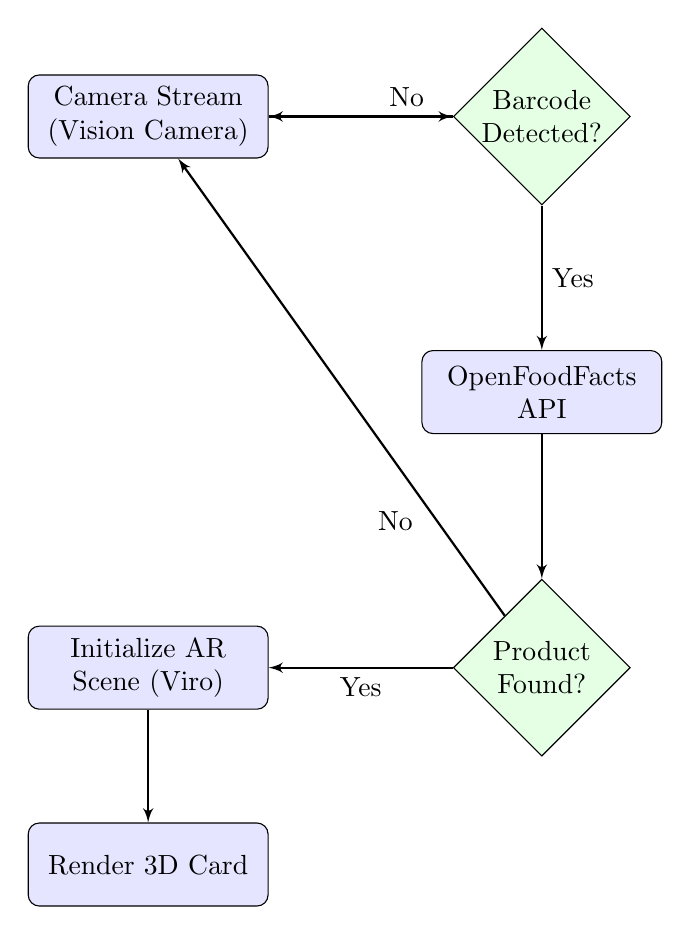
\begin{tikzpicture}[
    node distance=2.0cm,
    auto,
    block/.style={
        rectangle,
        draw,
        fill=blue!10,
        text width=8em,
        text centered,
        rounded corners,
        minimum height=3em
    },
    cloud/.style={
        draw,
        ellipse,
        fill=red!10,
        node distance=3cm,
        minimum height=2em
    },
    decision/.style={
        diamond,
        draw,
        fill=green!10,
        text width=4.5em,
        text badly centered,
        inner sep=0pt
    },
    line/.style={
        draw, -latex', thick
    }
]

    % Nodes
    \node [block] (camera) {Camera Stream (Vision Camera)};
    \node [decision, right of=camera, node distance=5cm] (scan) {Barcode Detected?};
    \node [block, below of=scan, node distance=3.5cm] (api) {OpenFoodFacts API};
    \node [decision, below of=api, node distance=3.5cm] (success) {Product Found?};
    \node [block, left of=success, node distance=5cm] (ar_init) {Initialize AR Scene (Viro)};
    \node [block, below of=ar_init, node distance=2.5cm] (render) {Render 3D Card};

    % Edges
    \path [line] (camera) -- (scan);
    \path [line] (scan) -- node [near start, above] {No} (camera);
    \path [line] (scan) -- node {Yes} (api);
    \path [line] (api) -- (success);
    \path [line] (success) -- node [near start] {No} (camera);
    \path [line] (success) -- node {Yes} (ar_init);
    \path [line] (ar_init) -- (render);

\end{tikzpicture}
\end{center}

\section{Testing Strategy}

To ensure the reliability of the application, I have incorporated \textbf{Jest} as the testing framework. Currently, the testing strategy focuses on unit testing the critical logic, specifically the data normalization and parsing functions.

Since the application relies heavily on external data from OpenFoodFacts, it is crucial to verify that the \texttt{buildFullName} logic and other utility functions handle various data shapes and edge cases correctly.

\textit{Note: The test suite will be expanded to include snapshot testing for UI components and integration tests for the scanner flow in future iterations.}

\section{Implementation Details}

\subsection{Managing the Camera Conflict}
One of the most significant technical hurdles was the conflict between \texttt{react-native-vision-camera} and \texttt{ViroReact}. Both libraries attempt to adhere to the device's camera resource exclusively.

Running them simultaneously results in a race condition where one library fails to initialize or the camera stream freezes.

\textbf{Solution}:
I implemented a strict state-machine approach. The \texttt{App.tsx} component manages a \texttt{appMode} state:

\begin{lstlisting}[language=Javascript]
type AppMode = "SCANNING" | "AR_VIEW";
const [appMode, setAppMode] = useState<AppMode>("SCANNING");

// Conditional Rendering
{appMode === "SCANNING" ? (
    <Camera ... />
) : (
    <ViroARSceneNavigator ... />
)}
\end{lstlisting}

By conditionally rendering only one component tree at a time, I ensure that the camera resource is released by one library before being claimed by the other. This ``handoff'' is managed with a slight delay (\texttt{setTimeout}) to allow for proper cleanup of native handles.

\subsection{AR Layout Strategy}
Positioning text and images in 3D space is fundamentally different from 2D web layout. Flexbox is supported by Viro but behaves inconsistently compared to standard CSS.

To achieve a stable, ``glassmorphism'' card layout:
\begin{itemize}
    \item \textbf{ViroFlexView}: Used as the main container for the card. It provides a bounded 2D surface within the 3D world.
    \item \textbf{Absolute Sizing}: Instead of relying on percentage-based responsiveness (which is ambiguous in 3D), I use fixed coordinate units for width and height.
    \item \textbf{Materials}: A custom \texttt{glassCard} material was created using a transparent black diffuse color (\texttt{rgba(20, 20, 20, 0.9)}) combined with constant lighting to ensure readability regardless of the environment's lighting conditions.
\end{itemize}

\subsection{Data Normalization}
Data from OpenFoodFacts can be inconsistent. The app implements a robust normalization layer (\texttt{buildFullName}, \texttt{fetchOpenFoodFacts}) that:
\begin{itemize}
    \item Prioritizes specific fields (e.g., \texttt{image\_front\_url} over \texttt{image\_url}).
    \item Sanitizes allergen tags (removing \texttt{en:} prefixes).
    \item Provides fallbacks for missing data (e.g., ``Unknown Product'' placeholders).
\end{itemize}

\section{Conclusion}
GrocARy demonstrates the viability of high-utility AR applications built with web technologies. By combining the raw performance of native modules for scanning with the immersive capabilities of ViroReact, and backing it with the massive OpenFoodFacts dataset, the application delivers a seamless user experience.

The architecture is designed to be extensible. Future work could re-introduce a lightweight backend for user favorites or caching, but the current serverless architecture serves the MVP goals perfectly: fast, reliable, and maintenance-free.

\end{document}
